\PassOptionsToPackage{unicode=true}{hyperref} % options for packages loaded elsewhere
\PassOptionsToPackage{hyphens}{url}
\documentclass[12pt,ignorenonframetext,aspectratio=169]{beamer}
\IfFileExists{pgfpages.sty}{\usepackage{pgfpages}}{}
\setbeamertemplate{caption}[numbered]
\setbeamertemplate{caption label separator}{: }
\setbeamercolor{caption name}{fg=normal text.fg}
\beamertemplatenavigationsymbolsempty
\usepackage{lmodern}
\usepackage{amssymb}
\usepackage{amsmath}
\usepackage{ifxetex,ifluatex}
\usepackage{fixltx2e} % provides \textsubscript
\ifnum 0\ifxetex 1\fi\ifluatex 1\fi=0 % if pdftex
  \usepackage[T1]{fontenc}
  \usepackage[utf8]{inputenc}
\else % if luatex or xelatex
  \ifxetex
    \usepackage{mathspec}
  \else
    \usepackage{fontspec}
\fi
\defaultfontfeatures{Ligatures=TeX,Scale=MatchLowercase}






%
\fi

  \usetheme[]{iqss}






% use upquote if available, for straight quotes in verbatim environments
\IfFileExists{upquote.sty}{\usepackage{upquote}}{}
% use microtype if available
\IfFileExists{microtype.sty}{%
  \usepackage{microtype}
  \UseMicrotypeSet[protrusion]{basicmath} % disable protrusion for tt fonts
}{}


\newif\ifbibliography


\hypersetup{
      pdftitle={Farm efficiency measures},
        pdfauthor={Deependra Dhakal},
          pdfborder={0 0 0},
    breaklinks=true}
%\urlstyle{same}  % Use monospace font for urls







% Prevent slide breaks in the middle of a paragraph:
\widowpenalties 1 10000
\raggedbottom

  \AtBeginPart{
    \let\insertpartnumber\relax
    \let\partname\relax
    \frame{\partpage}
  }
  \AtBeginSection{
    \ifbibliography
    \else
      \let\insertsectionnumber\relax
      \let\sectionname\relax
      \frame{\sectionpage}
    \fi
  }
  \AtBeginSubsection{
    \let\insertsubsectionnumber\relax
    \let\subsectionname\relax
    \frame{\subsectionpage}
  }



\setlength{\parindent}{0pt}
\setlength{\parskip}{6pt plus 2pt minus 1pt}
\setlength{\emergencystretch}{3em}  % prevent overfull lines
\providecommand{\tightlist}{%
  \setlength{\itemsep}{0pt}\setlength{\parskip}{0pt}}

  \setcounter{secnumdepth}{0}


  \usepackage{booktabs}
  \usepackage{longtable}
  \usepackage{emptypage}
  \usepackage{array}
  \usepackage{multirow}
  \usepackage{wrapfig}
  \usepackage{float}
  \usepackage{colortbl}
  \usepackage{pdflscape}
  \usepackage{tabu}
  \usepackage{threeparttable}
  \usepackage{threeparttablex}
  \usepackage[normalem]{ulem}
  \usepackage{rotating}
  \usepackage{makecell}
  \usepackage{xcolor}
  \usepackage{tikz} % required for image opacity change
  \usepackage[absolute,overlay]{textpos} % for text formatting
  \usepackage[utf8]{inputenc}
  \usetikzlibrary{mindmap,arrows,shapes,positioning,shadows,trees}
  \usepackage[skip=2pt]{caption}

  % this font option is amenable for beamer
  \setbeamerfont{caption}{size=\tiny}


%% IQSS overrides
\iqsssectiontitle{Outline}

\AtBeginSection[]{
  \title{\insertsectionhead}
  {
    \definecolor{white}{rgb}{0.776,0.357,0.157}
    \definecolor{iqss@orange}{rgb}{1,1,1}
    \ifnum \insertmainframenumber > \insertframenumber
    \frame{
      \frametitle{\iqsssectiontitleheader}
      \tableofcontents[currentsection]
    }
    \else
    \frame{
      \frametitle{Backup Slides}
      \tableofcontents[sectionstyle=shaded/shaded,subsectionstyle=shaded/shaded/shaded]
    }
    \fi
  }
}

\AtBeginSubsection[]{}

%%


  \title[]{Farm efficiency measures}



  \author[
        Deependra Dhakal
    ]{Deependra Dhakal}

  \institute[
    ]{
    GAASC, Baitadi \and Tribhuwan University
    }

\date[
      \today
  ]{
      \today
        }

\begin{document}

% Hide progress bar and footline on titlepage
  \begin{frame}[plain]
  \titlepage
  \end{frame}



\hypertarget{meaning-and-definition}{%
\section{Meaning and definition}\label{meaning-and-definition}}

\begin{frame}{}
\protect\hypertarget{section}{}
\begin{itemize}
\tightlist
\item
  Some managers are able to generate more production or use fewer
  resources than their neighbors because they use their resources more
  efficiently.
\item
  A general definition for efficiency is the quantity or value of
  production achieved per unit of resource employed.
\end{itemize}

\[
\textrm{Efficiency} = \frac{\textrm{Production}}{\textrm{Resources used}}
\]

\begin{itemize}
\tightlist
\item
  If a comparison with other farms or with a budget goal shows that an
  operation has an adequate volume of resources but is not reaching its
  production goals, then some resources are not being used efficiently.
\end{itemize}
\end{frame}

\hypertarget{efficiency-measures-physical-efficiency}{%
\section{Efficiency measures: Physical
efficiency}\label{efficiency-measures-physical-efficiency}}

\begin{frame}{}
\protect\hypertarget{section-1}{}
\begin{itemize}
\tightlist
\item
  Physical efficiency assigns technical coefficients to various physical
  inputs.
\item
  These are typically the conversion rates of economically valuable
  products from inputs such as:

  \begin{itemize}
  \tightlist
  \item
    the rate at which seed, fertilizer, and water are converted into
    crops,
  \item
    the rate at which feed is turned into livestock products,
  \item
    kilograms of grain harvested per acre,
  \item
    pigs weaned per sow, and
  \item
    litres of milk sold per cow
  \end{itemize}
\end{itemize}
\end{frame}

\begin{frame}{}
\protect\hypertarget{section-2}{}
\begin{enumerate}
\tightlist
\item
  Land use efficiency
\end{enumerate}

\begin{itemize}
\tightlist
\item
  Yield per acre (production efficiency):
  \(\frac{\textrm{Yield of the crop in the given farm}}{\textrm{Average yield of the locality}} \times 100\).
\item
  Crop yield index: It is a measure by which the yields of all crops on
  a given farm are compared with the average yields of these crops in
  the locality.
\item
  Intensity of cropping:
  \(\frac{\textrm{Area cropped}}{\textrm{Total cultivated area}}\times 100\).
\item
  System Index:
  \(\frac{\textrm{Potential net income per ha on farm}}{\textrm{Average standard net income per hectare in the area}} \times 100\)
\end{itemize}
\end{frame}

\begin{frame}{}
\protect\hypertarget{section-3}{}
\begin{enumerate}
\setcounter{enumi}{1}
\tightlist
\item
  Labor efficiency measures
\end{enumerate}

\begin{itemize}
\tightlist
\item
  A productive man equivalency is the average amount of work
  accomplished by one man in the usual eight hour day (man day).
\item
  Measures of labor efficiency are: crop acres per man or per man-year,
  livestock maintained per man or per man-year.
\item
  Gross profits per man or per man-year.
\end{itemize}
\end{frame}

\begin{frame}{}
\protect\hypertarget{section-4}{}
\begin{enumerate}
\setcounter{enumi}{2}
\tightlist
\item
  Machinery efficiency measures
\end{enumerate}

\begin{itemize}
\tightlist
\item
  Helpful in judging the accomplishment of the farm machinery and
  equipment for making changes in their investment it required. A list
  of some common measures of machinery efficiency is given below:

  \begin{itemize}
  \tightlist
  \item
    Machinery and equipment cost per cropped acre: Only, total annual
    costs are considered including repairs, fuel, depreciation, etc. in
    estimating the cost.
  \item
    Investment in machinery and equipment per crop acre.
  \end{itemize}
\end{itemize}
\end{frame}

\hypertarget{efficiency-measures-financial-efficiency}{%
\section{Efficiency measures: Financial
efficiency}\label{efficiency-measures-financial-efficiency}}

\begin{frame}{}
\protect\hypertarget{section-5}{}
\begin{itemize}
\tightlist
\item
  The financial portion of a complete farm analysis is designed to
  measure the solvency and liquidity of the business and to identify
  weakness in structure or mix of the various types of assets and
  liabilities.
\item
  The balance sheet and the income statement are the primary sources of
  data for calculating the measures related to the financial position of
  the business.
\end{itemize}
\end{frame}

\begin{frame}{}
\protect\hypertarget{section-6}{}
\begin{center}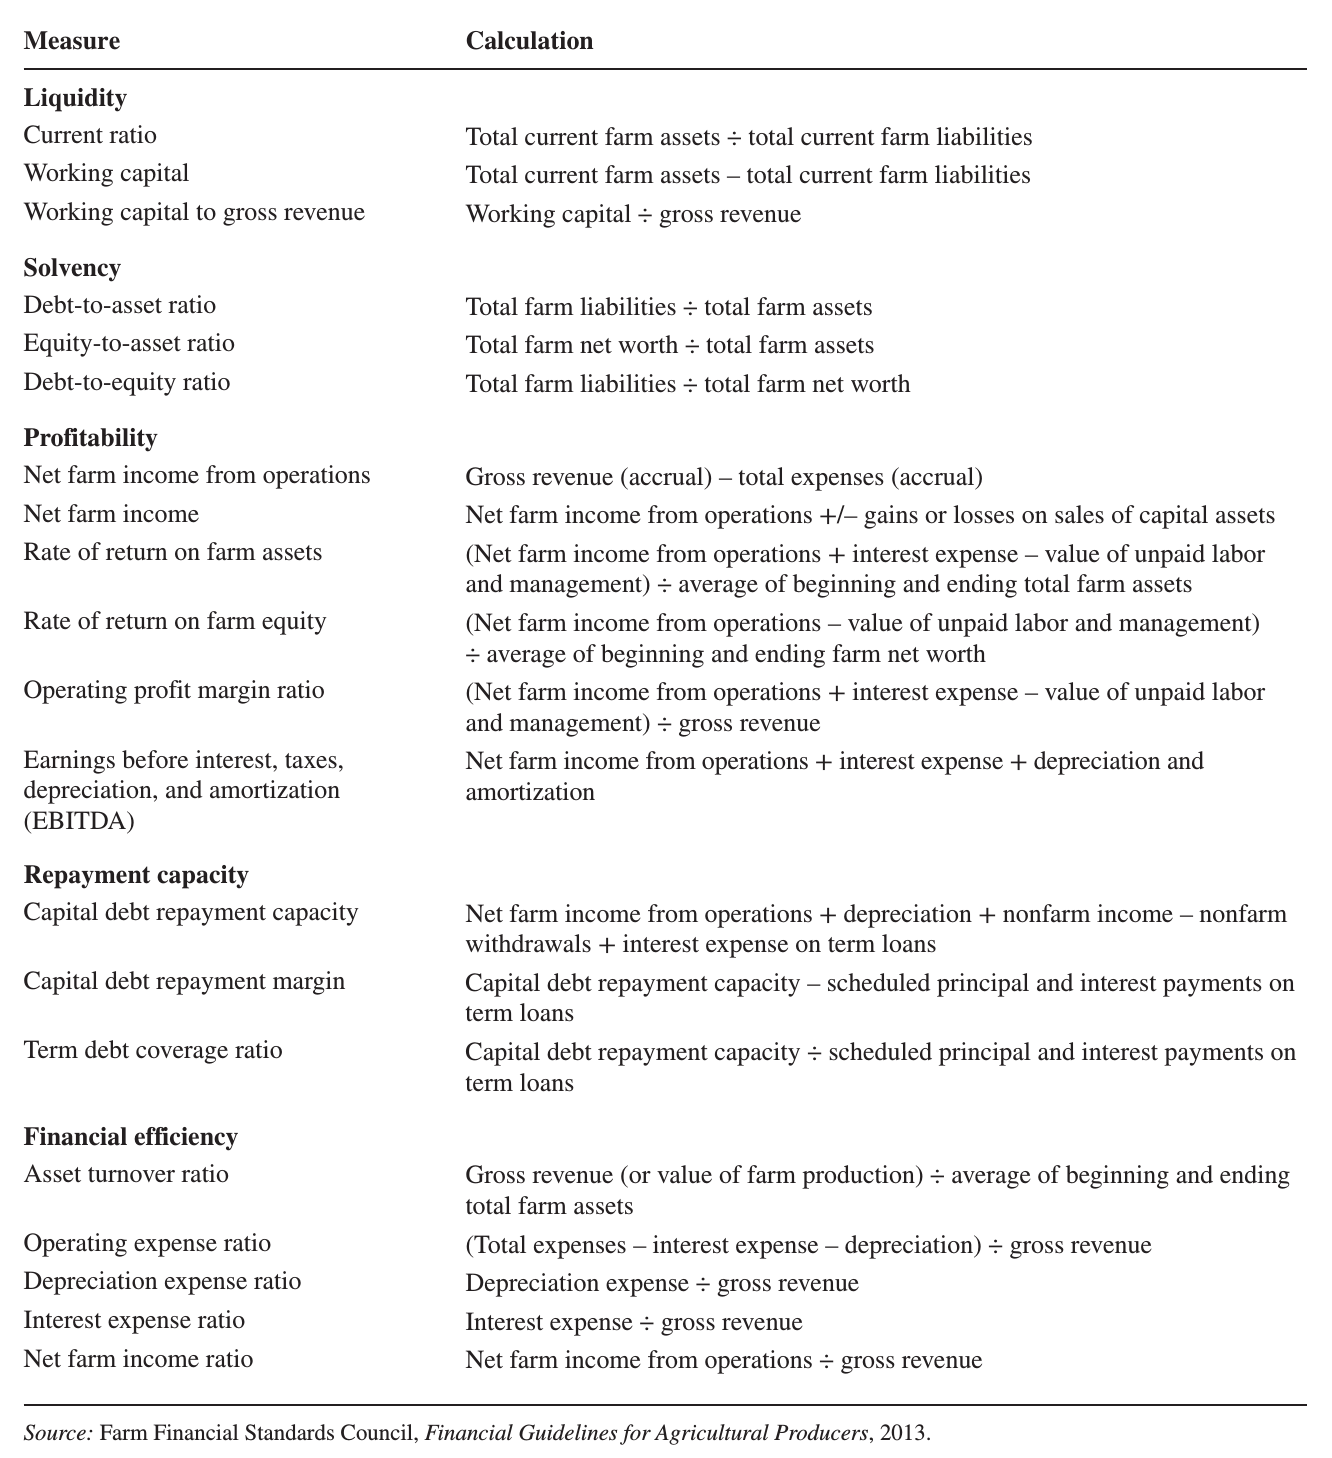
\includegraphics[width=0.5\linewidth]{./figs/farm_financial_ratios} \end{center}
\end{frame}

\begin{frame}{Solvency}
\protect\hypertarget{solvency}{}
\begin{itemize}
\tightlist
\item
  Solvency refers to the value of assets owned by the business compared
  to the amount of liabilities, or the relation between debt and equity
  capital. It also refers to what would be left in case all the assets
  are converted into cash and debts paid.
\item
  Solvency ratios:

  \begin{enumerate}
  \tightlist
  \item
    Leverage ratio/debt equity ratio:
    \(\frac{\textrm{Total liabilities}}{\textrm{Net worth}}\). Higher
    the leverage ratio, the farm operator has larger debt to pay in
    relation to his farm equity.
  \item
    Net capital ratio:
    \(\frac{\textrm{Total assets}}{\textrm{Total liabilities}}\). A
    greater than one NCR indicates that the liquidation of farm business
    would generate adequate cash to repay the total liabilities.
  \item
    Working ratio:
    \(\frac{\textrm{Working assets + Current assets}}{\textrm{Medium term liabilites + Current liabilities}}\).
  \end{enumerate}
\end{itemize}
\end{frame}

\begin{frame}{Liquidity ratios}
\protect\hypertarget{liquidity-ratios}{}
\begin{itemize}
\tightlist
\item
  These indicate the ability of the farmer to generate sufficient cash
  in order to meet the debt obligations without disrupting his farm
  business. These are:

  \begin{enumerate}
  \tightlist
  \item
    Current ratio/Acid test ratio:
    \(\frac{\textrm{Current assets}}{\textrm{Current liabilities}}\).
    This ratio indicates the extent to which current assets if
    liquidated would cover the current liabilities. i.e.~the value of
    current assets for each rupee of current liability. It reflects the
    adequacy of cash, accounts receivables to cover all the liabilities.
    Higher the value of current ratio, more liquidity exists in the farm
    business.
  \item
    Debt structure ratio:
    \(\frac{\textrm{Current liabilities}}{\textrm{Total liabilitites}}\).
    Lower the ratio, higher the liquidity position of farm.
  \end{enumerate}
\end{itemize}
\end{frame}

\hypertarget{economic-efficiency-capital-efficiency-physical-efficiency}{%
\section{Economic efficiency (Capital efficiency + Physical
efficiency)}\label{economic-efficiency-capital-efficiency-physical-efficiency}}

\begin{frame}{}
\protect\hypertarget{section-7}{}
\begin{center}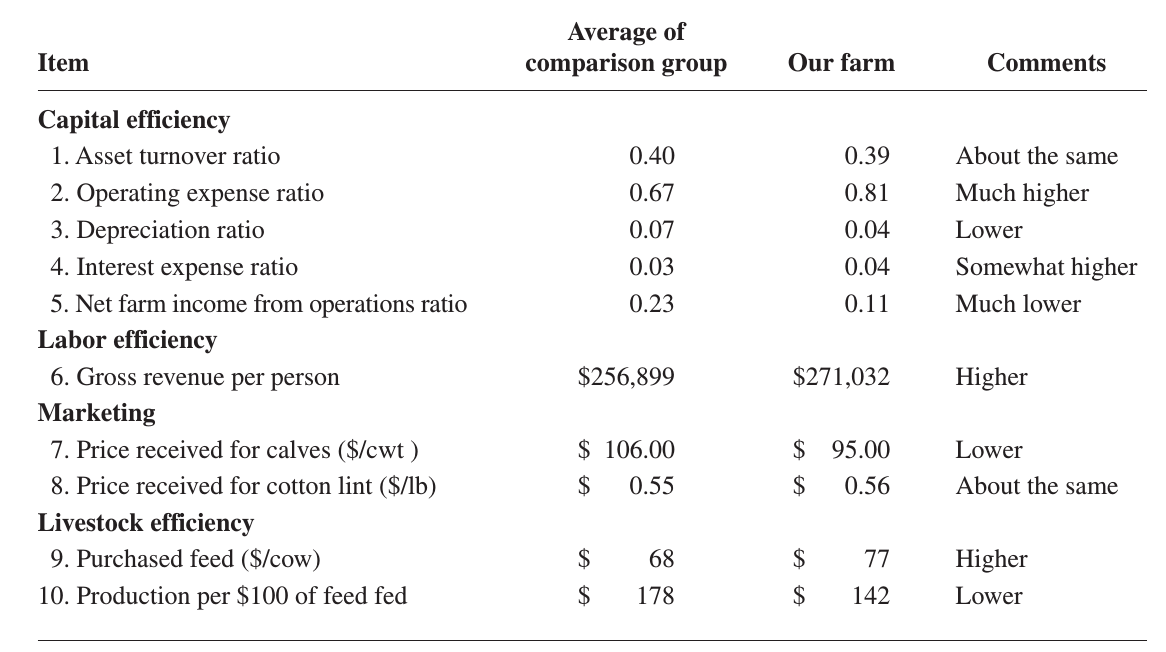
\includegraphics[width=0.8\linewidth]{./figs/farm_economic_efficiency_ratios} \end{center}
\end{frame}

\begin{frame}{Asset turnover ratio}
\protect\hypertarget{asset-turnover-ratio}{}
\footnotesize

\begin{itemize}
\tightlist
\item
  Measures how efficiently capital invested in farm assets is being
  used.
\item
  Found by dividing gross revenue generated by market value of total
  farm assets.
\item
  For e.g.~an asset turnover ratio of 0.25 indicates that gross revenue
  for one year was equal to 25 percent of the total capital invested in
  business. At this rate, it would take four years to produce
  agricultural products with a value equal to the total assets.
\item
  The operating profit margin ratio is a measure of profitability per
  unit produced. When the two are multiplied, they equate the rate of
  return on farm assets.
\end{itemize}

\[
ATR \times OMPR = ROA
\]

\begin{itemize}
\tightlist
\item
  So, overall profitability can be improved by: producing more units of
  output while maintaining the same profit margin per unit or by
  producing the same output but with a larger profit margin, or both.
\end{itemize}
\end{frame}

\begin{frame}{Operating expense ratio}
\protect\hypertarget{operating-expense-ratio}{}
\begin{itemize}
\tightlist
\item
  It is one of the four operational ratios are recommend to show what
  percent of gross revenue went for operating expenses, depreciation,
  interest, and net income.
\item
  The operating expense ratio is computed by dividing total operating
  expenses (excluding depreciation) by gross revenue.
\item
  Farms with a high proportion of rented land and machinery or hired
  labor will tend to have higher operating expense ratios.
\end{itemize}
\end{frame}

\begin{frame}{Depreciation expnese ratio}
\protect\hypertarget{depreciation-expnese-ratio}{}
\begin{itemize}
\tightlist
\item
  This ratio is computed by dividing total depreciation expense by gross
  revenue.
\item
  Farms with a relatively large investment in newer machinery,
  equipment, and buildings will have higher depreciation expense ratios.
\item
  A higher-than-average ratio may indicate underused capital assets.
\end{itemize}
\end{frame}

\begin{frame}{Interest expense ratio}
\protect\hypertarget{interest-expense-ratio}{}
\begin{itemize}
\tightlist
\item
  Total farm interest expense (adjusted for accrued interest payable at
  the beginning and end of the year) is divided by gross revenue to find
  this ratio.
\item
  Ratios higher than average, or higher than desired, may indicate too
  much dependence on borrowed capital or high interest rates on existing
  debt.
\end{itemize}
\end{frame}

\begin{frame}{Net farm income from operations ratio}
\protect\hypertarget{net-farm-income-from-operations-ratio}{}
\begin{itemize}
\tightlist
\item
  Dividing net farm income from operations by gross revenue measures
  what percent of gross revenue is left after paying all expenses (but
  before substracting any opportunity costs).
\item
  These four operational ratios will sum to 1.0 or 100 percent.
\item
  They can also be calculated using the value of farm production as a
  base instead of gross revenue.
\item
  In that case, the cost of purchased feed and livestock should not be
  included in operating expenses.
\end{itemize}
\end{frame}




\end{document}
